%\begin{frame}{Ablation: robustness to diverse skewed label densities}
%\end{frame}

\begin{frame}{Could LDS + FDS help when label distribution is skewed with one or more Gaussian peaks?}
	\begin{itemize}\setlength\itemsep{1.5em}
		\item Experimental setup
		\begin{itemize}
			\item Curated skewed label distributions with 1-4 Gaussian peaks on IMDB-WIKI-DIR
			\item Compared with vanilla model
		\end{itemize}
		\item Findings
		\begin{itemize}
			\item Robustness to distribution change
			\item Brings improvement
		\end{itemize}
	\end{itemize}
\end{frame}

\begin{frame}{Skewed label distribution with one Gaussian peak}
	\begin{figure}[h]
		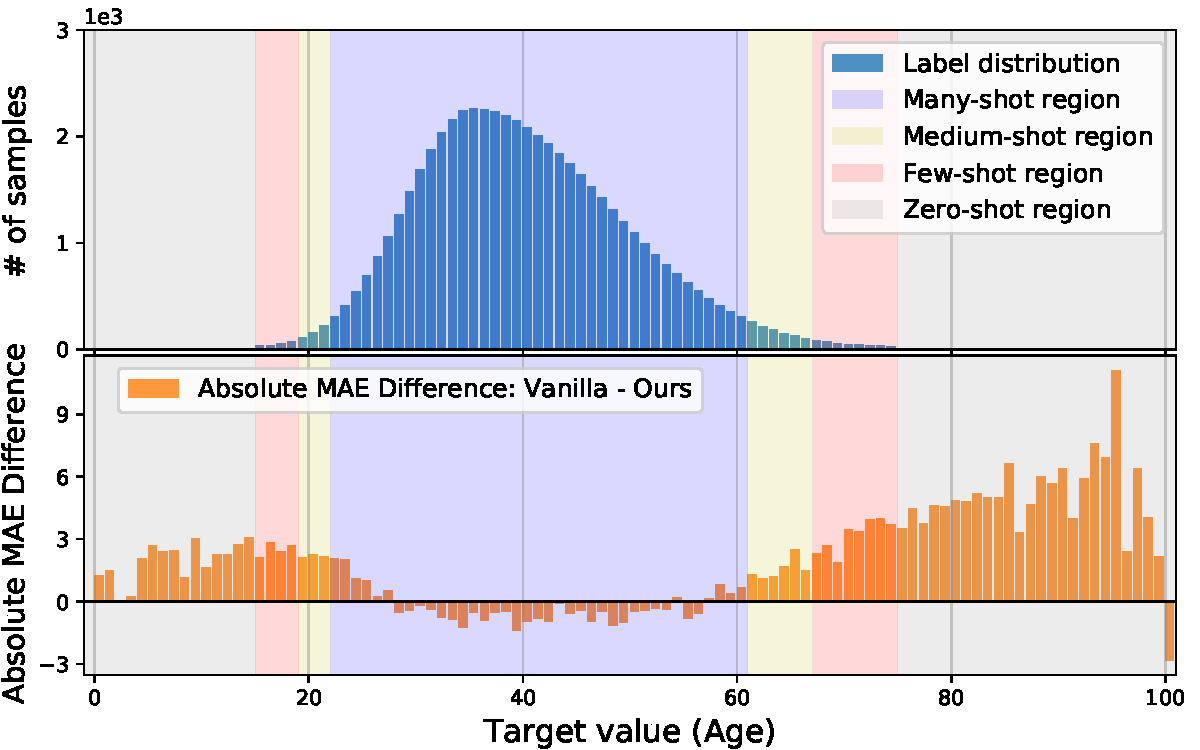
\includegraphics[width=0.7\linewidth]{images/interp_extrap_diff_peak1.pdf}
		\caption{MAE gains of LDS + FDS over vanilla model.}
	\end{figure}
	\begin{itemize}
		\item Performance gains, esp. for extrapolation \& interpolation
	\end{itemize}
	\credit{Image}{yang2021delving}
\end{frame}

\begin{frame}{Skewed label distribution with two Gaussian peaks}
	\begin{figure}[h]
		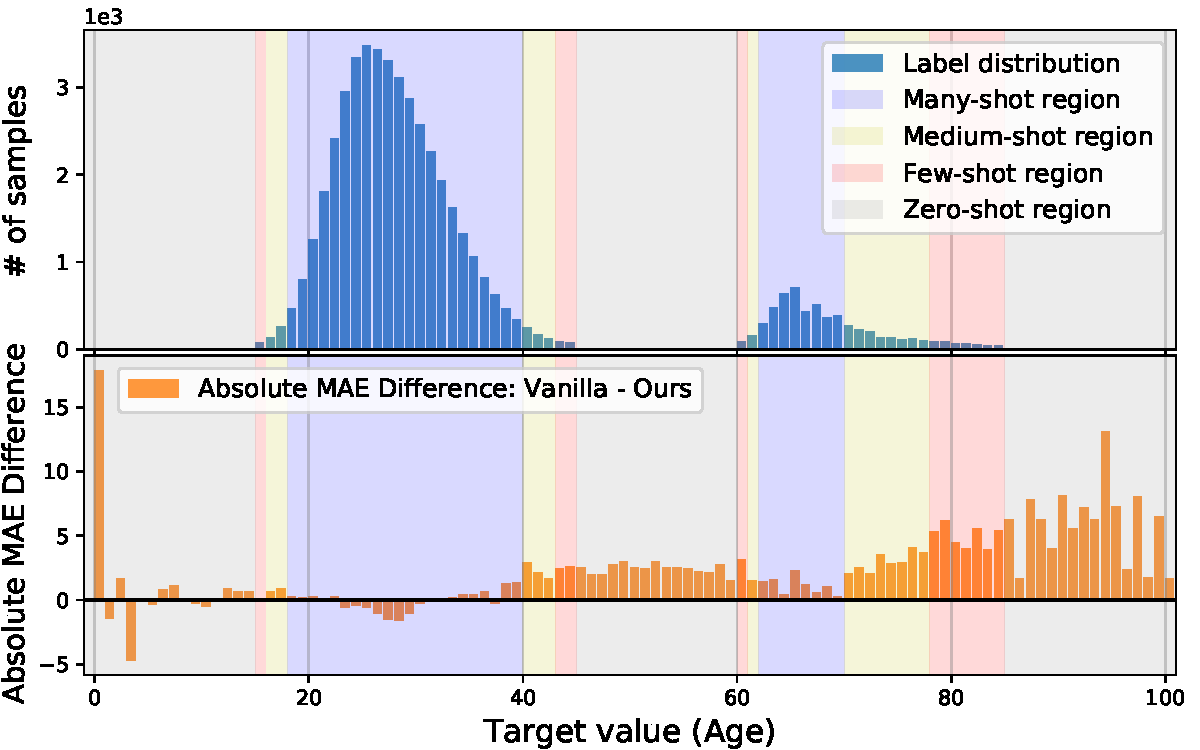
\includegraphics[width=0.7\linewidth]{images/interp_extrap_diff_peak2.pdf}
		\caption{MAE gains of LDS + FDS over vanilla model.}
	\end{figure}
	\begin{itemize}
		\item Performance gains, esp. for extrapolation \& interpolation
	\end{itemize}
	\credit{Image}{yang2021delving}
\end{frame}

\begin{frame}{Skewed label distribution with three Gaussian peaks}
	\begin{figure}[h]
		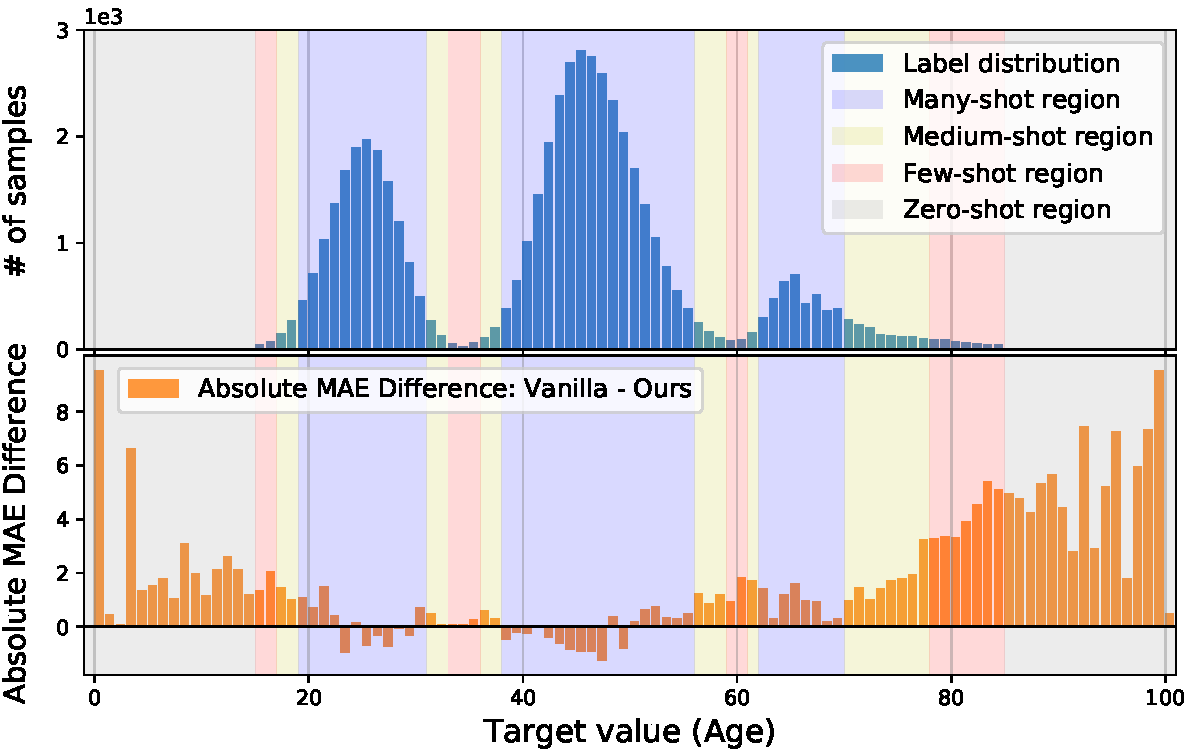
\includegraphics[width=0.7\linewidth]{images/interp_extrap_diff_peak3.pdf}
		\caption{MAE gains of LDS + FDS over vanilla model.}
	\end{figure}
	\begin{itemize}
		\item Performance gains, esp. for extrapolation \& interpolation
	\end{itemize}
	\credit{Image}{yang2021delving}
\end{frame}

\begin{frame}{Skewed label distribution with four Gaussian peaks}
	\begin{figure}[h]
		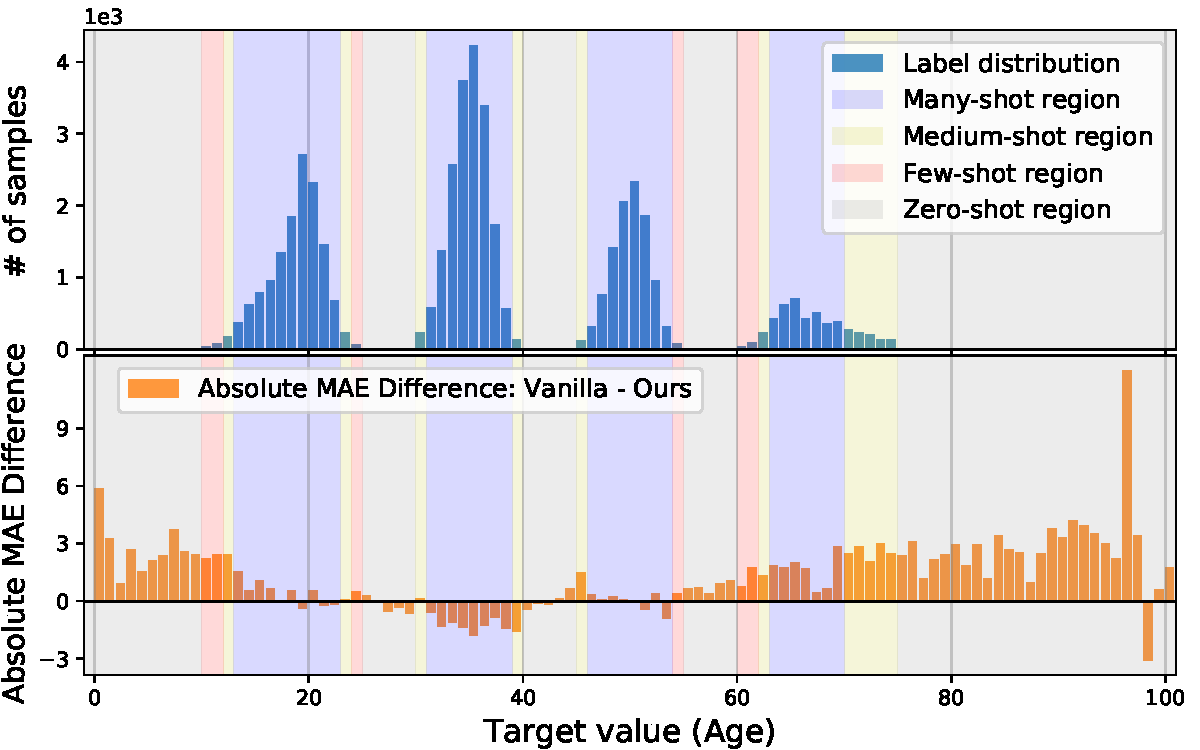
\includegraphics[width=0.7\linewidth]{images/interp_extrap_diff_peak4.pdf}
		\caption{MAE gains of LDS + FDS over vanilla model.}
	\end{figure}
	\begin{itemize}
		\item Performance gains, esp. for extrapolation \& interpolation
	\end{itemize}
	\credit{Image}{yang2021delving}
\end{frame}

\begin{frame}{Skewed label distribution with two Gaussian peaks on IMDB-WIKI-DIR}
	\begin{table}[t]
		\setlength{\tabcolsep}{1.5pt}
		\small
		\begin{center}
			\resizebox{\textwidth}{!}{
				\begin{tabular}{l|cccc|cccc}
					\toprule[1.5pt]
					Metrics      & \multicolumn{4}{c|}{MAE~$\downarrow$}       & \multicolumn{4}{c}{GM~$\downarrow$}    \\ \midrule
					Shot         & All   & w/ data  & Interp. & Extrap.   & All   & w/ data  & Interp. & Extrap.   \\ \midrule\midrule
					\textsc{Vanilla}      & 11.72 & 9.32 & 16.13  & 18.19 & 7.44 & 5.33 &  14.41  & 16.74 \\ \midrule\midrule
					\textsc{Vanilla} + \textbf{\textsc{LDS}} &  10.54 &  8.31  &    14.14 & 17.38  & 6.50  & 4.67  & 12.13 & 15.36 \\[1.2pt]
					\textsc{Vanilla} + \textbf{\textsc{FDS}} & 11.40 & 8.97 & 15.83  & 18.01  & 7.18  & 5.12 & 14.02 & 16.48 \\[1.2pt]
					\textsc{Vanilla} + \textbf{\textsc{LDS}} + \textbf{\textsc{FDS}} & \textbf{10.27} & \textbf{8.11}  & \textbf{13.71} & \textbf{17.02}  & \textbf{6.33} & \textbf{4.55}  & \textbf{11.71}  & \textbf{15.13}  \\ \midrule\midrule
					\textsc{\textbf{Ours~(best)} vs. Vanilla}   & \textcolor{darkgreen}{\textbf{+1.45}} & \textcolor{darkgreen}{\textbf{+1.21}} & \textcolor{darkgreen}{\textbf{+2.42}} & \textcolor{darkgreen}{\textbf{+1.17}} & \textcolor{darkgreen}{\textbf{+1.11}} & \textcolor{darkgreen}{\textbf{+0.78}} & \textcolor{darkgreen}{\textbf{+2.70}} & \textcolor{darkgreen}{\textbf{+1.61}} \\
					\bottomrule[1.5pt]
				\end{tabular}
			}
		\end{center}
		\caption{Interpolation \& extrapolation results}
	\end{table}
	\begin{itemize}
		\item Best results by smoothing both label \& feature distributions
	\end{itemize}
	\credit{Table}{yang2021delving}
\end{frame}

\begin{frame}{Different skewed label distributions on IMDB-WIKI-DIR}
	\begin{table}[t]
		\setlength{\tabcolsep}{4.5pt}
		\label{table:appendix-skewed-dist}
		\small
		\begin{center}
			\resizebox{0.95\textwidth}{!}{
				\begin{tabular}{l|ccccccc|ccccccc}
					\toprule[1.5pt]
					Metrics      & \multicolumn{7}{c|}{MAE~$\downarrow$}       & \multicolumn{7}{c}{GM~$\downarrow$}    \\ \midrule
					Shot         & All   & Many & Med. & Few & Zero & Interp. & Extrap.   & All   & Many & Med. & Few & Zero & Interp. & Extrap.   \\ \midrule\midrule
					\multicolumn{9}{l}{\emph{\textbf{1 peak:}}} \\ \midrule
					\textsc{Vanilla}       & 11.20 & 6.05 & 11.43 & 14.76 & 22.67 & $-$ & 22.67 & 7.02 & \textbf{3.84} & 8.67 & 12.26 & 21.07 & $-$ & 21.07 \\ [1.2pt]
					\textsc{Vanilla} + \textbf{\textsc{LDS}}  & 10.09 & 6.26 & 9.91 & 12.12 & 19.37 & $-$ & 19.37 & 6.14 & 3.92 & 6.50 & 8.30 & 16.35 & $-$ & 16.35 \\[1.2pt]
					\textsc{Vanilla} + \textbf{\textsc{FDS}}  & 11.04 & \textbf{5.97} & 11.19 & 14.54 & 22.35 & $-$ & 22.35 & 6.96 & \textbf{3.84} & 8.54 & 12.08 & 20.71 & $-$ & 20.71 \\[1.2pt]
					\textsc{Vanilla} + \textbf{\textsc{LDS}} + \textbf{\textsc{FDS}}  & \textbf{10.00} & 6.28 & \textbf{9.66} & \textbf{11.83} & \textbf{19.21} & $-$ & \textbf{19.21} & \textbf{6.09} & 3.96 & \textbf{6.26} & \textbf{8.14} & \textbf{15.89} & $-$ & \textbf{15.89}  \\ \midrule\midrule
					\multicolumn{9}{l}{\emph{\textbf{2 peaks:}}} \\ \midrule
					\textsc{Vanilla}      & 11.72 & 6.83 & 11.78 & 15.35 & 16.86 & 16.13  & 18.19 & 7.44 & 3.61 & 8.06 & 12.94 &15.21&  14.41  & 16.74 \\ [1.2pt]
					\textsc{Vanilla} + \textbf{\textsc{LDS}} &  10.54  & 6.72 & 9.65 & 12.60 & 15.30&   14.14 & 17.38  & 6.50    & 3.65 & \textbf{5.65} & 9.30 & 13.20 & 12.13 & 15.36 \\[1.2pt]
					\textsc{Vanilla} + \textbf{\textsc{FDS}} & 11.40  & 6.69 & 11.02 & 14.85 & 16.61 & 15.83  & 18.01  & 7.18   & \textbf{3.50} & 7.49 & 12.73 & 14.86 & 14.02 & 16.48 \\[1.2pt]
					\textsc{Vanilla} + \textbf{\textsc{LDS}} + \textbf{\textsc{FDS}} & \textbf{10.27}  & \textbf{6.61} & \textbf{9.46} & \textbf{11.96} & \textbf{14.89} & \textbf{13.71} & \textbf{17.02}  & \textbf{6.33}   & 3.54 & 5.68 & \textbf{8.80} & \textbf{12.83} & \textbf{11.71}  & \textbf{15.13}  \\ \midrule\midrule
					\multicolumn{9}{l}{\emph{\textbf{3 peaks:}}} \\ \midrule
					\textsc{Vanilla}      & 9.83  & 7.01 & 9.81 & 11.93 & 20.11 & $-$ & 20.11 & 6.04 & 3.93 & 6.94 & 9.84 & 17.77 & $-$ & 17.77 \\ [1.2pt]
					\textsc{Vanilla} + \textbf{\textsc{LDS}} & 9.08 & \textbf{6.77} & 8.82 & 10.48 & 18.43 & $-$ & 18.43 & \textbf{5.35} & \textbf{3.78} & 5.63 & 7.49 & 15.46 & $-$ & 15.46 \\[1.2pt]
					\textsc{Vanilla} + \textbf{\textsc{FDS}} & 9.65 & 6.88 & 9.58 & 11.75 & 19.80 & $-$ & 19.80 & 5.86 & 3.83 & 6.68 & 9.48 & 17.43 & $-$ & 17.43 \\[1.2pt]
					\textsc{Vanilla} + \textbf{\textsc{LDS}} + \textbf{\textsc{FDS}} & \textbf{8.96} & 6.88 & \textbf{8.62} & \textbf{10.08} & \textbf{17.76} & $-$ & \textbf{17.76} & 5.38  & 3.90 & \textbf{5.61} & \textbf{7.36} & \textbf{14.65} & $-$ & \textbf{14.65}  \\ \midrule\midrule
					\multicolumn{9}{l}{\emph{\textbf{4 peaks:}}} \\ \midrule
					\textsc{Vanilla}      & 9.49 & 7.23 & 9.73 & 10.85 & 12.16 & 8.23 & 18.78 & 5.68 & 3.45 & 6.95 & 8.20 & 9.43 & 6.89 & 16.02 \\ [1.2pt]
					\textsc{Vanilla} + \textbf{\textsc{LDS}} & 8.80 & \textbf{6.98} & 8.26 & 10.07 & 11.26 & 8.31 & \textbf{16.22} & 5.10 & \textbf{3.33} & \textbf{5.07} & 7.08 & 8.47 & 6.66 & \textbf{12.74} \\[1.2pt]
					\textsc{Vanilla} + \textbf{\textsc{FDS}} & 9.28 & 7.11 & 9.16 & 10.88 & 11.95 & 8.30 & 18.11 & 5.49 & 3.36 & 6.35 & 8.15 & 9.21 & 6.82 & 15.30 \\[1.2pt]
					\textsc{Vanilla} + \textbf{\textsc{LDS}} + \textbf{\textsc{FDS}} & \textbf{8.76} & 7.07 & \textbf{8.23} & \textbf{9.54} & \textbf{11.13} & \textbf{8.05} & 16.32 & \textbf{5.05} & 3.36 & \textbf{5.07} & \textbf{6.56} & \textbf{8.30} & \textbf{6.34} & 13.10  \\ 
					\bottomrule[1.5pt]
				\end{tabular}
			}
		\end{center}
	\end{table}
	\credit{Table}{yang2021delving}
\end{frame}
